\documentclass[./skripsi.tex]{subfiles}
\begin{document}
\chapter{Tinjauan Pustaka dan Landasan Teori}

\section{Tinjauan Pustaka}\label{bab2:tinjauanpustaka}
\par Beberapa penelitian tentang metode sistem pendeteksian intrusi telah dilakukan oleh peneliti-peneliti di bidang keamanan jaringan. Beberapa diantaranya menggunakan metode matematis statistik dan metode \textit{machine learning}.
\par Pada Penelitian \cite{zhang2001hide}, tentang pendeteksian menggunakan metode statistik dan  \textit{Neural Network} pada Intrusion Detection System untuk pendeteksian intrusi pada sisi serangan protokol UDP. Pengujian dilakukan dengan menggunakan beberapa jenis neural network antara lain Perceptron, Backpropagation, PBH, Fuzzy ARTMAP, dan Radial-based Function.
\par Akurasi tertinggi dicapai oleh Backpropagation, dan PBH (Perceptron Backpropagation Hybrid), dimana MSR errornya berkurang seiring dengan jumlah data yang dimasukkan yang berkisar di 5\% sampai 10\% dari intensitas data background.
\par Pada penelitian \cite{wirawan2015penerapan}, tentang penerapan kecerdasan buatan pada IDS.Penelitian ini menggunakan salah satu metode Machine Learning yakni Naive Bayes memperoleh akurasi sebesar 89\% dengan running time. Penelitian ini menerapkan \textit{Naive Bayes Classifier} dengan memilah atribut berdasarkan korelasi, dan menggunakan mean/standar deviasi untuk atribut kontinyu pada 3-interval dan 5-interval. Metode ini memperoleh akurasi sebesar 89\% dengan running time rata-rata 31 detik.
\par Pada Penelitian \cite{jacobus2014penerapan}, tentang penerapan metode Support Vector Machine pada Intrusion Detection System secara Realtime menerapkan 3 kelas untuk proses pendeteksian jenis intrusi yakni normal, probe, dan DoS. Untuk beberapa tipe intrusi dapat terdeteksi dengan akurasi diatas 90\%, dengan memanfaatkan kluster pada beberapa jenis faktor parameter dari header packet yang diperoleh dari hasil data mining.
\par Penelitian-penelitian sebelumnya banyak menggunakan metode matematis tanpa diintegrasikan dengan sistem pendeteksi intrusi yang umum dipakai contohnya seperti \textit{snort IDS}. Hal ini menyebabkan kurangnya implementasi praktis yang terjadi pada sistem pendeteksi intrusi yang harusnya diimplementasikan metode-metode pada penelitian tersebut.
\par Untuk mengatasi masalah ini. Pada penelitian ini akan diterapkan metode \textit{Deep Learning} yang akan dijadikan prototip integrasi sistem pendeteksi intrusi dengan aplikasi modern. Metode \textit{Deep Learning} yang akan digunakan adalah CNN dan LSTM. Metode ini menggabungkan \textit{time series regression} pada LSTM dan memanfaatkan fungsi CNN yang dapat mendeteksi pola berdasarkan jarak relatif piksel.
\par Dataset yang akan digunakan pada penelitian ini berasal dari dataset CTU yang terdiri dari beberapa botnet, yang baik secara trafik penyebaran data maupun konten data memiliki ciri khusus \textit{malware}.
\par Metode CNN digunakan karena dataset \textit{payload} memiliki keacakan data tinggi namun memiliki pola yang serupa secara relatif. Metode LSTM digunakan karena keacakan data dalam bentuk \textit{time series}. Penelitian ini diharapkan mampu mengintegrasikan sistem pendeteksi intrusi dengan metode \textit{filter} jaringan berbasis CNN dan \textit{profiler} jaringan berbasis LSTM.

\section{Landasan Teori}\label{bab2:landasanteori}
\subsection{Protocol Data Unit}
\par \textit{Protocol Data Unit} atau dapat disingkat PDU merupakan satuan unit yang ditransmisikan antar \textit{node} pada jaringan. PDU terdiri dari \textit{control information} dan \textit{user data}. Dalam arsitektur standarisasi ISO untuk protokol komunikasi, setiap layer mengimplementasikan protokol yang disesuaikan dengan tipe atau mode pertukaran data tertentu.
\par Protokol TCP atau \textit{Transmission Control Protocol} menerapkan mode transfer berorientasi koneksi, dan PDU pada protokol ini disebut segmen, sedangkan pada protokol UDP atau \textit{Unit Datagram Protocol} memiliki PDU yang disebut datagram untuk transfer data secara \textit{connectionless}. Pada layer \textit{network}, PDU disebut paket, terlepas dari jenis muatannya.
\begin{figure}%[H]
    \centering
    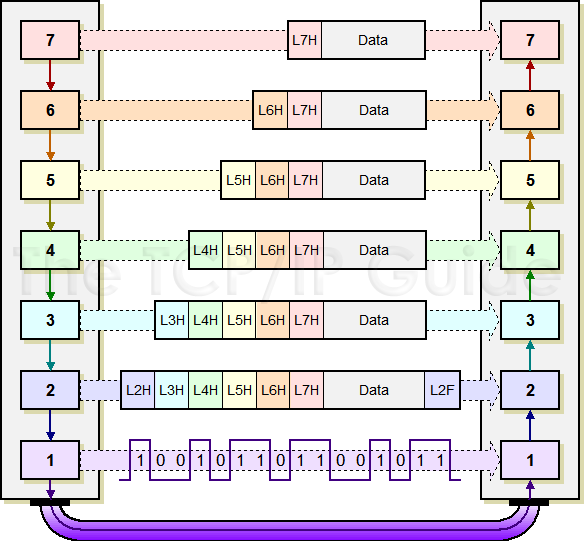
\includegraphics[width=0.5\textwidth]{public/assets/img/osidataenkapsulasi.png}
    \caption{Packet Data Unit pada OSI Layer}
    \label{fig:pduosi}
\end{figure}
\par Berdasarkan gambar \ref{fig:pduosi}, setiap protokol memiliki bentuk PDU nya masing-masing. Diagram diatas menunjukkan layer 7 PDU yang terdiri dari L7H dan data. Ketika data di teruskan ke layer 6, data ditambahkan dengan L6H sehingga menjadi layer 6 PDU, dan seterusnya sampai di layer 1 data dengan seluruh header di transmisikan. Data yang dapat diperoleh dari MTU
\par Data pada jaringan berbentuk \textit{ethernet frame} dengan ukuran \textit{Maximum Transmission Unit} (MTU) tiap frame sebesar 1500 bytes. Untuk transmisi data lebih besar dari 1500 bytes akan dilakukan pemecahan per frame.
\subsection{IDS}
\par Sistem deteksi intrusi (IDS) adalah perangkat atau aplikasi perangkat lunak yang memantau jaringan atau sistem untuk aktivitas jahat atau pelanggaran kebijakan. Setiap aktivitas atau pelanggaran berbahaya biasanya dilaporkan kepada administrator atau dikumpulkan secara terpusat menggunakan sistem informasi keamanan dan manajemen kejadian (SIEM). Sistem SIEM menggabungkan output dari berbagai sumber, dan menggunakan teknik penyaringan alarm untuk membedakan aktivitas berbahaya dari alarm palsu. \cite{martellini2017cyber}
\par Tipe IDS berkisar dalam ruang lingkup dari satu komputer ke jaringan besar. \cite{axelsson2000intrusion} Klasifikasi yang paling umum adalah sistem deteksi intrusi jaringan (NIDS) dan sistem deteksi intrusi berbasis host (HIDS). Sistem yang memantau file sistem operasi penting adalah contoh dari HIDS, sedangkan sistem yang menganalisis lalu lintas jaringan yang masuk adalah contoh dari NIDS. Dimungkinkan juga untuk mengklasifikasikan IDS dengan pendekatan deteksi: varian yang paling terkenal adalah deteksi berbasis tanda tangan (mengenali pola-pola buruk, seperti malware); dan deteksi berbasis anomali (mendeteksi penyimpangan dari model lalu lintas "baik", yang sering bergantung pada pembelajaran mesin), yang lain adalah deteksi berbasis reputasi (mengenali potensi ancaman sesuai dengan skor reputasi). Beberapa produk IDS memiliki kemampuan untuk menanggapi intrusi yang terdeteksi. Sistem dengan kemampuan respons biasanya disebut sebagai sistem pencegahan intrusi. \cite{newman2009computer} Sistem deteksi intrusi juga dapat melayani tujuan tertentu dengan menambahkannya dengan alat khusus, seperti menggunakan honeypot untuk menarik dan mengkarakterisasi lalu lintas berbahaya.
\cite{liao2013intrusion}
\subsection{Snort IDS}\label{bab2:snortids}
Snort adalah sistem deteksi intrusi jaringan open source (IDS) dan sistem pencegahan intrusi (IPS) \cite{carr2007snort} yang dibuat pada tahun 1998 oleh Martin Roesch, pendiri dan mantan CTO Sourcefire. \cite{greenemeier2006sourcefire} Snort sekarang dikembangkan oleh Cisco, yang membeli Sourcefire pada 2013.
\subsubsection{Cara kerja Snort IDS}\label{bab2:carakerjasnortids}
\par Sistem deteksi / pencegahan intrusi (IDS / IPS) berbasis jaringan sumber terbuka milik Snort memiliki kemampuan untuk melakukan analisis lalu lintas waktu-nyata dan pendataan paket pada jaringan Internet Protocol (IP). Snort melakukan analisis protokol, pencarian konten, dan pencocokan.

\par SnortIDS dapat digunakan untuk mendeteksi probe atau serangan. Baik intrusi berupa \textit{fingerprinting} sistem operasi,  serangan URL, buffer overflows, probe SMB, dan \textit{port scanning}. Karena bersifat \textit{open source} snortIDS banyak dikembangkan dan dijadikan \textit{engine} dasar untuk membangun IDS. \cite{stanger2011cheat}

\par Snort dapat dikonfigurasi dalam tiga mode utama: sniffer, packet logger, dan deteksi intrusi jaringan. Dalam mode sniffer, program akan membaca paket jaringan dan menampilkannya di konsol. Dalam mode packet logger, program akan mencatat paket-paket ke disk. Dalam mode deteksi intrusi, program akan memonitor lalu lintas jaringan dan menganalisanya terhadap aturan yang ditetapkan oleh pengguna. Program kemudian akan melakukan tindakan spesifik berdasarkan apa yang telah diidentifikasi.
\begin{figure}%[H]
    \centering
    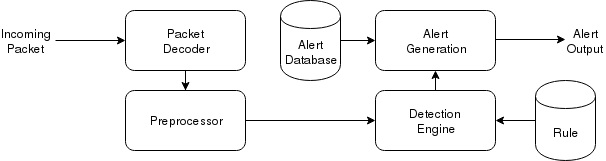
\includegraphics[width=0.8\textwidth]{public/assets/img/SnortIDS.png}
    \caption{Sistem kerja Snort IDS}
    \label{fig:sissnort}
\end{figure}
\par Berdasarkan gambar sistem kerja \ref{fig:sissnort}, dapat diketahui bahwa sistem \textit{preprocessor} berada setelah \textit{packet decoder} dan sebelum \textit{detection engine}. \textit{Preprocessor} pada snort berperan dapat sekaligus sebagai \textit{packet decoder} dan \textit{detection engine}. \textit{Preprocessor} memiliki argumen yang mengacu kepada \textit{detection engine} dan membaca \textit{packet} yang sudah di decode seperti pada URL agar dapat teratur ketika di deteksi pada \textit{detection engine}.
\subsection{Deep Learning}\label{bab2:deeplearning}
\par Banyak masalah dalam penerapan kecerdasan buatan adalah bahwa banyak faktor variasi yang dapat memengaruhi setiap bagian dari data yang dapat kita amati. Contohnya, masing-masing piksel dalam gambar sebuah mobil merah mungkin menyerupai dengan mobil hitam saat di malam hari. Bentuk bayangan mobil tergantung pada sudut pandang. Sebagian besar penerapan kecerdasan buatan mengharuskan kita untuk memisahkan faktor-faktor variasi dan membuang faktor-faktor yang dapat diabaikan.
\par Ekstraksi fitur abstrak sangat sulit dilakukan. Banyak faktor yang bervariasi seperti aksen pembicara pada ekstraksi fitur suara yang secara langsung mudah di kenali oleh manusia sedangkan jika diterapkan secara matematis justru sangat sulit dikenali.
\par Deep Learning memecahkan masalah ini pada saat proses merubah bentuk dengan mengekspresikan data dalam bentuk lain yang lebih sederhana dan mudah diamati secara matematis. Deep Learning memungkinkan komputer untuk membangun konsep kompleks yang dapat memprediksi hal yang dapat dikenali manusia.
\par Deep learning merupakan salah satu penerapan dari Machine Learning yang digunakan untuk memahami data yang memiliki makna. Contohnya seperti gambar, suara, maupun bentuk data lain yang dapat diinterpretasikan tidak secara matematis. Deep Learning memanfaatkan konsep matematis pada Machine Learning untuk mempelajari data yang lebih kompleks. nyata.\cite{goodfellow2016deep}
\subsection{Jaringan Syaraf Tiruan}\label{bab2:jst}
\par Jaringan saraf tiruan atau JST dipandang di sini sebagai model komputasi paralel, dengan berbagai tingkat kompleksitas, terdiri dari unit pemrosesan adaptif yang saling berhubungan. Jaringan ini adalah implementasi paralel halus dari sistem statis atau dinamis nonlinear. 
\par Fitur yang sangat penting dari jaringan ini adalah sifat adaptifnya, di mana "belajar dengan contoh" menggantikan "pemrograman" tradisional dalam menyelesaikan masalah. Fitur ini membuat model komputasi sangat cocok pada sistem yang memiliki sedikit atau pemahaman tidak lengkap atas masalah yang harus dipecahkan tetapi di mana data pelatihan tersedia.
\par Fitur utama lainnya adalah paralelisme intrinsik yang memungkinkan perhitungan solusi yang cepat ketika jaringan ini diimplementasikan pada komputer digital paralel atau, pada akhirnya, ketika diimplementasikan dalam perangkat keras khusus. \cite{hassoun1995fundamentals}
\subsection{Botnet}
\par Botnet merupakan sekumpulan program yang saling terhubung dan biasanya mengirimkan pesan spam atau berpartisipasi dalam melakukan DDoS. Botnet menyerang protokol yang menyediakan kanal komunikasi seperti protokol HTTP, IRC, dan Email.
\subsection{CNN}\label{bab2:cnn}
\par CNN merupakan salah satu metode artificial neural network yang biasa diterapkan untuk data dalam bentuk gambar. Pada CNN data gambar melalui proses ekstraksi fitur. Pada proses ekstraksi fitur setiap piksel dari gambar akan diubah dalam bentuk data matriks angka. Fitur yang sudah diekstraksi kemudian akan di alirkan melalui dua layer yaitu \textit{convolutional layer} dan \textit{pooling layer}.
\par Convolutional layer terdiri dari neuron yang tersusun sehingga membentuk sebuah filter yang memiliki ukuran lebar, tinggi, dan tebal piksel. Contohnya ukuran \textit{convolutional layer} 5x5x3, memiliki panjang 5 piksel, tinggi 5 piksel dan tebal 3 yang merupakan channel dari gambar dalam bentuk representasi RGB.
\par Filter ini kemudian akan digeser ke seluruh bagian dari gambar yang kemudian akan di lakukan operasi perkalian antara input dan nilai dari filter sehingga menghasilkan output yang disebut \textit{feature map}. Parameter pada convolutional layer, salah satunya adalah Stride. Stride adalah parameter yang menentukan jumlah pergeseran filter. Jika nilai stride 1, maka filter akan bergeser sebanyak 1 piksel.
\par Semakin kecil stride maka akan semakin detil informasi yang diperoleh dari input. Padding merupakan parameter yang menentukan jumlah piksel (bernilai 0) yang akan ditambahkan di setiap sisi dari input. Hal ini digunakan dengan tujuan untuk memanipulasi output dari feature map. Pooling Layer merupakan layer CNN yang berada setelah Convolutional Layer. Pooling layer merupakan sebuah filter yang bergeser juga pada seluruh area feature map.
\par Pada setiap pergeseran filter, nilai maksimum akan diambil sebesar ukuran dari filter. Contoh apabila menggunakan max pooling 2x2 dengan stride 2
maka setiap pergeseran filter, nilai maksimum pada area 2x2 akan dipilih, sedangkan Average Pooling memilih nilai rata-rata. Berikut ini adalah contoh sederhana bentuk \textit{Convolutional Neural Network}
\begin{figure}%[H]
    \centering
    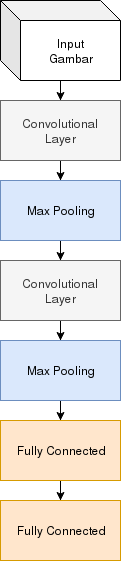
\includegraphics[width=0.35\linewidth]{public/assets/img/SimpleCNN.png}
    \caption{Model CNN sederhana}
    \label{fig:modelcnnsederhana}
\end{figure}
\par Berdasarkan gambar \ref{fig:modelcnnsederhana} dapat diketahui sederhananya model CNN memiliki komponen dasar yakni \textit{Convolutional Layer}, \textit{Max Pooling}, dan \textit{Fully Connected Layer}. Pada \textit{Convolutional Layer} volume akan diperkecil seiring dengan dimasukannya input pada Layer ini. Misal dijabarkan persamaan sebagai berikut.
\begin{equation}
    V_1 = W_1 \times H_1 \times D_1
    \label{eq:volcnn}
\end{equation}
\par Berdasarkan persamaan \ref{eq:volcnn}, diketahui $W_1$ merupakan lebar gambar $H_1$ merupakan tinggi gambar, dan $D_1$ merupakan \textit{deepthness} gambar yang menunjukan komponen RGB dari gambar. Agar dapat dimasukkan pada CNN harus memiliki beberapa \textit{hyperparameter} yang dibutuhkan antara lain. 
\par $K$ = jumlah filter, $F$ = \textit{spatial extents}, $S$ = \textit{stride}, dan $P$ = jumlah \textit{zero padding}. Maka akan dihasilkan volume $V_2$
\begin{equation}
    V_2 = W_2 \times H_2 \times D_1
    \label{eq:volcnn2}
\end{equation}
Dengan parameter persamaan \ref{eq:volcnn2} diperoleh dari :
\begin{equation}
    W_2 = (W_1 - F + 2P)/S + 1
    \label{eq:w2cnn}
\end{equation}
\begin{equation}
    H_2 = (H_1 - F + 2P)/S + 1
    \label{eq:h2cnn}
\end{equation}
\begin{equation}
    D_2 = K
    \label{eq:d2cnn}
\end{equation}
\par Dapat dilihat dari persamaan \ref{eq:w2cnn} dan \ref{eq:h2cnn} bahwa ukuran $W_2$ dan $H_2$ akan tetap simetris ketika dimasukkan dalam CNN.
\begin{figure}%[H]
    \centering
    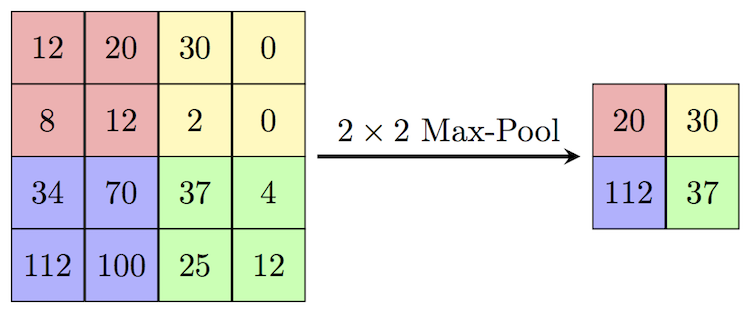
\includegraphics[width=0.5\textwidth]{public/assets/img/MaxpoolSample2.png}
    \caption{Max Pooling Layer}
    \label{fig:maxpool}
\end{figure}
\par Berdasarkan gambar \ref{fig:maxpool}, pada layer \textit{max pooling} ukuran akan direduksi kembali dan sesuai dengan ketentuan \textit{stride} dan ukuran kernel yan akan diambil nilai terbesarnya.
\par Kemudian pada layer aktivasi akan diaktivasi dapat menggunakan aktivasi \textit{sigmoid}, aktivasi \textit{relu}, atau aktivasi lainnya.
\subsection{LSTM} 
\par LSTM (Long short-term memory) memiliki kemampuan untuk melupakan informasi yang tidak relevan pada jaringan RNN (recurrent neural network). LSTM merupakan RNN yang terdiri dari 4 bagian yakni, cell state, input gate, output gate, dan forget gate. Cell state merupakan bobot dari hidden layer. Input gate merupakan jalur nilai input datang. Forget gate merupakan jalur yang berfungsi untuk meniadakan atau melupakan informasi yang datang. Output gate merupakan jalur keluaran berdasarkan cell state setelah forget gate dilewati.

\begin{figure}%[H]
    \centering
    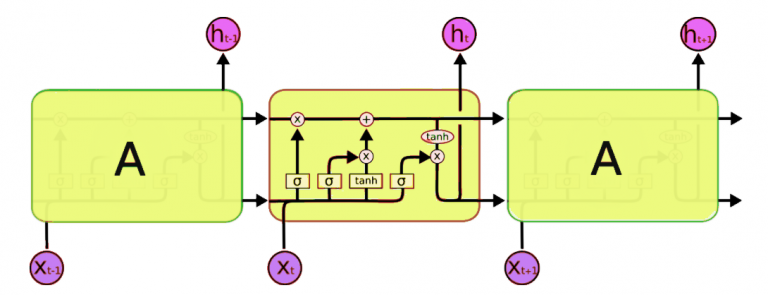
\includegraphics[width=0.8\textwidth]{public/assets/img/LSTM1.png}
    \caption{Layer LSTM}
    \label{fig:lstm1}
\end{figure}

\par Berdasarkan gambar \ref{fig:lstm1}, sebuah sel \textit{Long Short Term Memory} terdiri dari empat komponen yakni komponen gate \textit{input gate}, \textit{output gate}, dan \textit{forget gate}, dan juga komponen \textit{cell state}. Keempat komponen ini masing-masing memiliki perannya sendiri. Setiap peran yang ada pada komponen ini yang membuat LSTM dapat lebih di andalkan dalam proses pendeteksian data sekuensial.

\subsubsection{Forget Gate}\label{bab2:lstmforgetgate}
\par \textit{Forget Gate} bertanggung jawab untuk menghapus informasi dari status sel. Informasi yang tidak lagi diperlukan untuk LSTM atau informasi yang kurang penting dihapus melalui gerbang ini. Hal Ini diperlukan untuk mengoptimalkan kinerja jaringan LSTM.

\begin{figure}%[H]
    \centering
    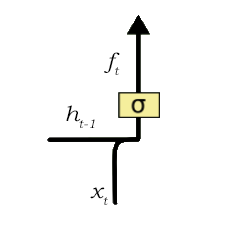
\includegraphics[width=0.4\textwidth]{public/assets/img/ForgetGate1.png}
    \caption{Forget Gate}
    \label{fig:lstm_forget_gate}
\end{figure}
\par Dapat dilihat dari gambar \ref{fig:lstm_forget_gate}, bahwa \textit{forget gate} menerima dua input $h_{t-1}$ dan $x_t$.  $h_{t-1}$ adalah keadaan tersembunyi dari sel sebelumnya atau output dari sel sebelumnya dan $x_t$ adalah input sesaat. gambar \ref{fig:lstm_forget_gate} diatas dapat dijabarkan oleh persamaan \textit{forget gate} berikut ini :
\begin{equation}
    f_t = \sigma (w_f[h_{t-1},x_t]+b_f)
    \label{eq:lstm_forget_gate}
\end{equation}

\par Dengan $f_t$ = \textit{forget gate}, $\sigma$ = fungsi sigmoid, $w_f$ = bobot dari forget gate, $h_{t-1}$ = output dari sel lstm sebelumnya saat $t-1$, $x_t$ = input dari waktu saat ini, $b_x$ = bias dari gate.
\par Berdasarkan persamaan \ref{eq:lstm_forget_gate}, input yang diberikan dikalikan dengan matriks bobot dan kemudian ditambahkan bias kemudian di masukkan pada fungsi sigmoid. Fungsi sigmoid menghasilkan vektor, dengan nilai mulai dari 0 hingga 1, sesuai dengan setiap angka dalam keadaan sel. 
\par Pada dasarnya, fungsi sigmoid bertanggung jawab untuk memutuskan nilai mana yang harus disimpan dan mana yang harus dibuang. Jika output dari \textit{forget gate} bernilai ‘0’ maka \textit{forget gate} akan melupakan keadaan sel melupakan informasi itu sepenuhnya. Sebaliknya, apabila output dari \textit{forget gate} bernilai '1' maka \textit{forget gate} akan mengingat seluruh informasi itu. Output vektor ini dari fungsi sigmoid dikalikan ke \textit{cell state}.

\subsubsection{Input Gate}\label{lstm:inputgate}
\par \textit{Input Gate} bertanggung jawab untuk penambahan informasi ke status sel. Penambahan informasi ini pada dasarnya adalah proses tiga langkah seperti yang terlihat dari diagram di atas.

\begin{figure}%[H]
    \centering
    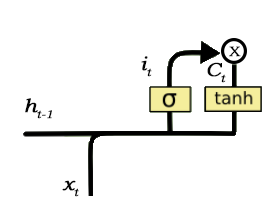
\includegraphics[width=0.5\textwidth]{public/assets/img/InputGate1.png}
    \caption{Input Gate}
    \label{fig:inputgate1.png}
\end{figure}

\par Berdasarkan Gambar \ref{fig:inputgate1.png}, \textit{input gate} memiliki parameter $h_{t-1}$ yang merupakan nilai \textit{hidden cell} dari waktu sebelumnya, dan $x_t$ yang merupakan nilai \textit{hidden cell} dari waktu sekarang, dan $\sigma$ yang merupakan fungsi aktivasi, sehingga dapat dijabarkan persamaan \textit{input gate} berikut ini :

\begin{equation}
    i_t = \sigma (w_i[h_{t-1},x_t] + b_i)
    \label{eq:lstm_input_gate}
\end{equation}
\par dengan $i_t$ = input gate, $\sigma$ = fungsi sigmoid, $w_i$ bobot dari input gate, $h_{t-1}$ = output dari sel lstm sebelumnya $t-1$, $x_t$ = input dari waktu saat ini, $b_i$ bias dari input gate.

\begin{enumerate}
    \item Mengatur nilai apa yang perlu ditambahkan ke keadaan sel dengan melibatkan fungsi sigmoid. Ini pada dasarnya sangat mirip dengan gerbang lupa dan bertindak sebagai filter untuk semua informasi dari $h_{t-1}$ dan $x_{t}$.
    \item Membuat vektor yang berisi semua nilai yang mungkin yang dapat ditambahkan (seperti yang dirasakan dari $h_{t-1}$ dan $x_t$. Hal ini dilakukan dengan menggunakan fungsi tanh, yang menampilkan nilai dari -1 hingga +1.
    \item Mengalikan nilai filter pengaturan (gerbang sigmoid) ke vektor yang dibuat (fungsi tanh) dan kemudian menambahkan informasi berguna ini ke \textit{cell state} melalui operasi penambahan.
    \item Setelah proses tiga langkah ini selesai, layer memastikan bahwa hanya informasi yang ditambahkan ke keadaan sel yang relevan.
\end{enumerate}
\subsubsection{Output Gate}\label{bab2:lstmoutputgate}

\begin{figure}%[H]
    \centering
    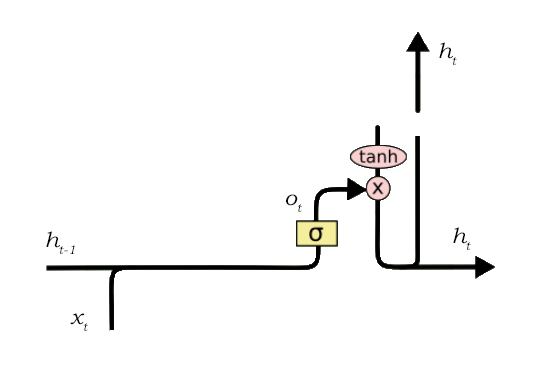
\includegraphics[width=0.5\textwidth]{public/assets/img/OutputGate1.png}
    \caption{Output Gate}
    \label{fig:lstm_output_gate}
\end{figure}
\par Berdasarkan gambar \ref{fig:lstm_output_gate}, \textit{output gate} menerima input dari $h_{t-1}$ dan $x_t$, yang langsung diaktivasi dengna fungsi sigmoid. Sehingga dapat dijabarkan persamaan untuk \textit{output gate} adalah sebagai berikut :
\begin{equation}
    o_t = \sigma (w_o[h_{t-1},x_t]+b_o)
    \label{eq:lstm_output_gate}
\end{equation}
\par Dengan $o_t$ = output gate, $\sigma$ = fungsi sigmoid, $w_o$ merupakan bobot dari \textit{output gate}, $h_{t-1}$ = output dari sel lstm sebelumnya $t-1$, $x_t$ = input dari waktu saat ini, $b_o$ = bias dari output gate. Berdasarkan persamaan \ref{eq:lstm_output_gate}, fungsi dari \textit{output gate} terbagi menjadi tiga langkah:
\begin{enumerate}
    \item Membuat vektor setelah menerapkan fungsi tanh ke status sel, sehingga menskalakan nilai ke rentang -1 hingga +1.
    \item Membuat filter menggunakan nilai-nilai $h_{t-1}$ dan $x_t$, sehingga dapat mengatur nilai-nilai yang perlu dikeluarkan dari vektor yang dibuat di atas. Filter ini lagi menggunakan fungsi sigmoid.
    \item  Mengalikan nilai filter pengaturan ini ke vektor yang dibuat pada langkah 1, dan mengirimkannya sebagai output dan juga ke keadaan tersembunyi sel berikutnya.
\end{enumerate}
\par Filter pada contoh di atas memastikan bahwa output mengurangi semua nilai lain kecuali nilai cell state. Oleh karena itu filter juga perlu dibuat pada input dan nilai-nilai \textit{hidden state} dan diterapkan pada vektor \textit{cell state}.
\cite{gers1999learning}

\subsection{Python}
\par Python merupakan bahasa pemrograman yang memiliki banyak \textit{library} yang memiliki banyak fungsi dan penerapan. Beberapa \textit{library} python antara lain seperti \textit{tensorflow} dan \textit{keras} yang merupakan framework yang digunakan untuk membuat model jaringan syaraf tiruan maupun \textit{machine learning}. Banyaknya \textit{library} python seperti tensorflow dan keras menyebabkan python sebagai salah satu bahasa pemrograman yang paling umum digunakan pada bidang data sains. 
\par Python banyak digunakan oleh \textit{Data scientist} untuk melakukan penelitian model kecerdasan buatan. Contohnya kegunaan \textit{library} keras yang biasa diterapkan pada jaringan syaraf tiruan.
\subsection{Flask}\label{bab2:flask}
\par Flask adalah framework web yang dibuat dengan Python. framework ini termasuk dalam kategori \textit{microservice} karena tidak memerlukan \textit{tools} atau \textit{library} tertentu atau dapat juga disebut dengan \textit{microframework}.
\par Flask tidak memiliki lapisan abstraksi untuk basis data, validasi formulir, dan juga tidak memiliki \textit{third-party library} yang menyediakan fungsi umum. Flask mendukung ekstensi yang dapat menambahkan fitur aplikasi sehingga dapat diimplementasikan dalam Flask itu sendiri. Ekstensi yang ada seperti \textit{Object Relational Mappers}, \textit{Form Validation}, dan \textit{upload handling}. Ekstensi flask lebih sering diperbaharui dari \textit{core} flask sendiri.
\subsection{Keras}
\par Keras adalah salah satu library python untuk jaringan syaraf tiruan. Keras merupakan \textit{framework} dari tensorflow, CNTK, atau Theano. Keras dikembangkan sebagai solusi untuk memungkinkan eksperimen jaringan syaraf tiruan dengan cepat. Keras memungkinkan peneliti lebih cepat mengaplikasikan idenya langsung dalam bentuk hasil yang di inginkan.
\end{document}
